
\section{はじめに}
% 警邏とは
所与の領域を1人または複数の巡査が動き回り,
その領域内の指定された場所を十分な頻度で訪問することを
警邏(patrolling)という\cite{chen2013fence, coene2011charlemagne, czyzowicz2011boundary}.


\red{「距離空間$M$の有限部分集合$V$が与えられる」などにする?}
本稿では,辺に非負の長さがついた無向グラフ$G$上を,
速さ$1$の巡査が何人かで動きまわることで,
多くの頂点が十分な頻度で訪問されるようにする問題を考える.
巡査$m$人による$G$上の運行とは,
各巡査$i \in \{1, \ldots, m\}$の
各時刻$t \in \Rset$における位置$a _i (t)$を定めたものをいう.
位置$a _i (t)$は$G$の頂点または辺上の一点であり,
任意の時刻$s$,$t$に対し,
$a _i (s)$と$a _i (t)$の間の$G$上での距離は$\abs{s - t}$を超えない.


$G$の各頂点には利得および{\timelimit}と呼ばれる非負整数が与えられている.
ある運行によって頂点$v$が警備されるとは,
$v$の{\timelimit}を$q$とするとき,
長さ$q$のどの時間区間を見ても,
いずれかの巡査が$v$を少くとも一度は訪問する
(すなわち任意の時刻$t \in \Rset$に対して
巡査$i$と時刻$\tau \in [t, t + q)$が存在し
$a _i (\tau) = v$)ことをいう.
運行$A$が頂点の集合$W$を警邏するとは,$A$が$W$の全頂点を警備することをいう.
$W$が巡査$m$人により警邏可能であるとは,
$W$を警邏する巡査$m$人による運行が存在することをいう.
\red{「警備」の多重定義}

本稿では次の問題を考える.

\begin{cooperativepatrollingproblem}
	巡査の人数$m$とグラフ$G$(辺の長さ,頂点の利得と{\timelimit}を含む)が
	与えられたとき,
	警邏可能な頂点集合のうち利得の和が最大となるものを求めよ.
\end{cooperativepatrollingproblem}

この問題は,巡査が一人かつ
全頂点の利得と{\timelimit}が等しい場合に限っても,
ハミルトン路問題からの帰着により
NP困難である\cite[Theorem~8]{coene2011charlemagne}.
そこでグラフの形状を限ったときにどのようになるかを調べる.

一つの頂点が複数の巡査の訪問により警備され得ることに注意されたい.
例えば図\ref{figure: }では,…….
\red{(←適当な例を図に描く。)}

Coeneら\cite{coene2011charlemagne}は似た問題を扱っているが,
このような協力を許さず,
各頂点を専ら一人の巡査が「担当」することを要求している.
つまり,各頂点$v \in W$が単独警備されること,すなわち
$v$によって決るある一人の巡査が,
$v$の{\timelimit}以上の長さのどの時間区間においても
$v$を訪問することを要求しているのである.
対比のため本稿ではこの問題を非協力警備問題と呼ぶことにする
(\cite{coene2011charlemagne}ではMPLPPと称している).
Coeneら\cite{coene2011charlemagne}の諸結果においては,
この非協力という限定が,
多項式時間算法の設計にも困難性の証明にも重要な役割を果している.
この限定を外したときの様子を調べるのが本稿の目的である.

%% 複数の巡査の協力を考える本稿の問題においては,
%% 巡査が1人の場合でNP困難性が示されていない
%% 線分・閉路の場合と星・木で全頂点の利得と{\timelimit}が等しい場合
%% が未解決である.

本稿ではグラフ$G$の形状として
線分,星と,枝の長さがすべて等しい完全グラフの3種類を扱うこととし
\red{(←定義が必要ですね。図にしましょうか。)},
以降はそれぞれを Line, Star, {\unit}と呼ぶ.
{\unit}は,その各辺の長さを$d$とすると,
同じ頂点数で辺の長さがすべて$d/2$というStarの特別な場合と考えることができる.

% 頂点の警備にかかるコストにはその頂点の{\timelimit}とその頂点までの移動距離という2種類の制約があるが,
% {\unit}はそのうち頂点までの移動距離が全頂点で等しいという場合となる.

%% 頂点の警邏を考える今回の問題においては,グラフの形状は頂点間の移動距離の性質としてのみ意味を持つ.

% 巡査協力なしの結果との比較

協力警邏問題についての我々の結果と,
非協力警邏問題についてのCoeneらの結果を,
グラフの形ごとに比較すると次のようになる.
それぞれ\ref{section: line},\ref{},\ref{}節で述べる.
\begin{itemize}
\item 
Lineでは,
非協力警邏問題は%巡査数・利得・{\timelimit}がすべて一般の場合であっても
動的計画法により多項式時間で解けることが
示されていた\cite[Theorem~11]{coene2011charlemagne}が,
その正しさは非協力の設定に強く依存している.
本稿では協力警邏問題について,
全頂点の{\timelimit}が等しい場合にはPであることを示す(定理\ref{theo:LineEqualTimelimit}).
\item
Starでは,
全頂点の利得と{\timelimit}がすべて等しい場合に限っても,
非協力警邏問題はNP困難であることが示されていた\cite[Theorem~10]{coene2011charlemagne}.
本稿では,この場合の協力警邏問題はPとなるという興味深い結果を得る(定理**).
なお利得または{\timelimit}を一般にすると,
巡査が一人であっても(したがって協力・非協力に関わらず)
NP困難であることがわかっている\cite[Theorems 5 and 6]{coene2011charlemagne}.
\item 
{\unit}では,
全頂点の{\timelimit}が等しい場合は\patrolling がPであることを示す(定理**).
Starでは全頂点の{\timelimit}が等しくても利得が一般だとNP困難になるので,
これにより{\unit}はStarよりも簡単に解ける場合となっていることが分かる.
\end{itemize}

Lineと{\unit}については
{\timelimit}が一般の場合については多項式時間アルゴリズムやNP困難性を示すのが難しかったため,
{\timelimit}の代わりに「{\interval}」というものを考え,
最初の訪問時刻から{\interval}ごとの時刻ちょうどに訪問し続けること
を警備の条件とする問題も考えた.




\subsection*{関連研究}

\red{(あまり本筋に関係ない関連研究は、論文冒頭ではなくこの辺に書くのも手)}

% 警邏に関する研究には様々な問題設定があり,
% 例えば線分や閉路のような交わりの無い1次元的な領域のすべての点を警邏する
% 塀の警邏(Fence Patrolling)問題~\cite{chen2013fence, czyzowicz2011boundary}や,
% より一般的なグラフで辺全体ではなく頂点を警備する警邏問題~\cite{coene2011charlemagne},
% グラフと巡査が与えられて警邏可能かを判定する問題だけでなく,
% 塀の警邏問題においてなるべく長い塀を警邏する問題~\cite{czyzowicz2011boundary}や
% 全体の訪問の待ち時間の最大値を最小化する問題~\cite{chen2013fence}
% なども考えられている.
% \red{(加筆予定)}

また,LineやStarは木の特別な場合である.



\section{Line}
\label{section: line}

グラフがLineの場合,
グラフの全体(辺と頂点)は実直線上にあるとし,
%実直線と同一視し,/ 
頂点の名前$v_1, v_2, \ldots, v_n$はその位置を表す実数値も表すことにする.

また,Lineの場合は順序保存運行というものを考えることができる.
運行$A$が順序保存であるとは,
$A$が定める巡査$u_1, u_2, \ldots, u_m$の位置$a_1, a_2, \ldots, a_m$が,
任意の時刻$t \in \Rset$において
$a_1(t) \leq a_2(t) \leq \cdots \leq a_m(t)$を満すことである.

% 頂点集合$W$を警備する任意の運行$A$に対して$A$が警備する頂点集合$W$を警備する順序保存運行$A'$が存在する.
巡査$m$人により警邏可能な任意の頂点集合$W$は,
巡査$m$人による或る順序保存運行$A'$によって警邏される.
%
これは次のように示すことができる.
%
まず$W$は警邏可能であるから,ある運行$A$が存在し$W$を警邏するとする.
$a_1, a_2, \ldots, a_m$を$A$が定める各巡査の位置,
$s_i : \Nset^m \to \Nset$を与えられた$m$個の整数のうち$i$番目に小さいものを返す関数として,
\[ a'_i(t) := s_i( a_1(t), a_2(t), \ldots, a_m(t) ) \]
のように$a'_1, a'_2, \ldots, a'_m$を定める.
巡査の最高速度は互いに等しいので,
各巡査$u_1, u_2, \ldots, u_m$の位置を$a'_1, a'_2, \ldots, a'_m$%により定める運行$A'$が存在する.

\red{これは運行となる.}
%

任意の時刻$t$において
$\set{ a_1(t), a_2(t), \ldots, a_m(t) } = \set{ a'_1(t), a'_2(t), \ldots, a'_m(t) }$
% また,各頂点がいずれかの巡査により訪問される時刻は$A$と$A'$で違いが無いので
であるから運行$A'$も$W$を警邏しており,
%
$a'_1(t) \leq a'_2(t) \leq \cdots \leq a'_m(t)$
であるから$A'$は順序保存運行である.


% 任意の警邏可能な頂点集合は或る順序保存運行$A$によって警邏される.
% 但し運行$A$が順序保存であるとは,
% $A$が定める巡査$u_1, u_2, \ldots, u_m$の位置$a_1, a_2, \ldots, a_m$が,
% 任意の時刻$t \in \Rset$において
% $a_1(t) \leq a_2(t) \leq \cdots \leq a_m(t)$を満すことである.



\red{2.1節と2.2節はまとめられそう?「なるべく右に」が共通なので説明をまとめられるかも。
「一番左の巡査をなるべく右に動かす」で解決できる場合とできない場合、という説明ができる。}


\subsection{{\timelimit}がすべて等しい場合}
\label{subsec:LineUnaryTimelimit}

\red{この設定に関しては、やはりCollins et al.との関係を述べるべきではないか?}



本節では次のことを示す.
% まず,{\timelimit}がすべて等しい場合は{\patrolling}は多項式時間で解くことができる.
% \red{←定理以上の情報を何も与えていない。こう書くくらいなら「本節では次のことを示す」などの方が良い。
% 他の可能性としては、何か全体の方向性を示す言葉、例えば現状2.2節冒頭に書いてある「この場合は協力が関係なくなるので」的なことを(うまく一言で言えそうなら)書くとか。}

\begin{theo}
	\label{theo:LineEqualTimelimit}
	グラフの形状がLineで{\timelimit}がすべて等しい場合,
	{\patrolling}は多項式時間で解くことができる.
\end{theo}

% ここでは

% 実際にはすべての頂点が単独警備される
% (すなわち任意の頂点$v$と時刻$t \in \Rset$に対して
% 	巡査$u_i$と時刻$\tau \in [t, t + q)$が存在し
% 	$a _i (\tau) = v$),
% ような警邏により最大の利得が得られる(


% これは,任意の警邏可能な頂点集合$W$に対して
% $W$を警邏する特別な運行が存在するので,
% そのような運行の中で利得が最大となるものを求めればよいためである
% (補題\ref{lemm:LineEqualTimelimitIndependentInterval}).
% \red{←今から定理\ref{theo:LineEqualTimelimit}の証明を始めるということがわかる言いまわしにしよう。}

初めに次の補題を示す.

\begin{lemm}
	\label{lemm:movableAreaofPatrolleronLine}
	頂点$v_i$がある1人の巡査$s$により単独警備されているとき
	% (すなわち任意の時刻$t \in \Rset$に対して
	% 時刻$\tau \in [t, t + q)$が存在し
	% $a _s (\tau) = v_i$)
	,
	{\timelimit}を$q_i$として,
		$s$は常に区間$[v_i - q_i/2, v_i + q_i/2]$にいる.
\end{lemm}
\red{↑「単独警備」はCoeneらの非協力警邏問題の定義に出て来たものであることを述べる。
  それを十分うまく述べれば多分、読者が「なるほど、Lineかつ$Q$一定のときは、要するに協力する意味がなくなったから
  簡単になったのだな」と(2.2節の冒頭には書いてあるが、既にこの時点で)
  自然に納得できるように書けるのでは?}

\begin{proof}[証明]
	\newcommand{\vout}{v_{\mathrm{out}}}
	この区間にない或る座標$\vout \notin [v_i - q_i/2, v_i + q_i/2]$を$s$が
	時刻$t_0$に訪問するとする.
	$\vout$と$v_i$の間の移動には
	少くとも時間$\lvert v_i - \vout \rvert > q _i / 2$を要するから,
	$s$は区間$[t_0 - q _i / 2, t_0 + q _i / 2]$に属する時刻に$v_i$を訪問できない.
	この区間の長さは$
		q_i
	$であるので,$s$が$v _i$を単独警備していることに反する.
\end{proof}



これにより次の補題が成り立つ.


\begin{lemm}
	\label{lemm:LineEqualTimelimitIndependentInterval}
	グラフの形状がLineで,全頂点の{\timelimit}がすべて$Q$であるとする.
	頂点集合$W$が警邏可能であるとする.
	このとき,
	$W$を警邏する
	運行であって,
        各巡査が$W$の頂点を左端とする長さ$Q / 2$の区間を往復するものが存在する.
    \red{人数?}
\end{lemm}


\begin{proof}[証明]

	\newcommand{\leftmostpoint}{v_l}
	\newcommand{\leftmostpatroller}{u_1}

	巡査数$m$に関する帰納法で示す.
	$m = 0$のときは明らかなので,以下$m > 0$とする.

	$m$人の巡査により警邏可能な頂点集合$W$が与えられたとき,
	\ref{section: line}章の初めで述べたように
	$W$を警邏する$m$人の巡査による{\orderedrun}$A$が存在する.
	$W$の頂点のうち最も左にあるものを$\leftmostpoint$とする.
\red{$A$名づけるタイミング?}

	まず,すべての巡査は$[\leftmostpoint, +\infty)$に存在するとしてよい.
	なぜなら,
	$\leftmostpoint$より左に存在することがある巡査は
	その時間$\leftmostpoint$で停止するようにしても,
	$W$は警邏されるためである.

	ここで,$\leftmostpoint$に注目する.
	いま,$A$は{\orderedrun}であり,どの巡査も$\leftmostpoint$より左には進まないので,
	一番左側を動く巡査$\leftmostpatroller$以外の巡査が$\leftmostpoint$に存在するときは,
	$\leftmostpatroller$も$\leftmostpoint$に存在する.
	よって$\leftmostpoint$は$\leftmostpatroller$により単独警備される.

	一方,$\leftmostpatroller$はこの区間を最高速度$1$で往復することで
	この区間に含まれるすべての頂点を警備することができる.
	実際,$\leftmostpatroller$がこのような往復をするとき
	$\leftmostpoint \leq x \leq \leftmostpoint + Q/2$
	である位置$x$に存在する時刻の間隔の最大値は
	\[
		\max( 2(x - \leftmostpoint), 2(\leftmostpoint + Q/2 - x) )
		\leq 2(\leftmostpoint + Q/2 - \leftmostpoint) = Q
	\]
	より,$[\leftmostpoint, \leftmostpoint + Q/2]$に含まれるどの頂点も
	{\timelimit}を超えずに訪問できていることが分かる.

	したがって,
	補題\ref{lemm:movableAreaofPatrolleronLine}より
	$\leftmostpatroller$が動ける範囲は
	$[\leftmostpoint, \leftmostpoint + Q/2]$に含まれるが
	% \red{(←これを使っているのは次段落の「$\leftmostpatroller$以外の巡査達によって警邏可能であったので」なのだから、それに近い位置に書く。)},
	
	よって,残りの巡査は
	$W ^- := \setmid{ v \in W }{ \leftmostpoint + Q/2 < v }$
	を警備すればよいことが分かる.

	$W ^-$の頂点はすべて$\leftmostpatroller$以外の巡査達
	%$S \setminus \set$\leftmostpatroller$$
	によって警邏可能であったので,
	帰納法の仮定より,
	巡査が$W ^-$の頂点を左端とする長さ$Q / 2$の区間を往復するようにできる.
	%は$W ^-$のうち最も左にある頂点$x_l^-$を左端とする長さ$Q / 2$の区間を往復するようにできる.
\end{proof}

補題\ref{lemm:LineEqualTimelimitIndependentInterval}により,各巡査の動きとしては
頂点の座標$v_i$を左端とする区間$[v_i, v_i + Q/2]$を往復するもののみを考えれば良い.
$n$個の区間$I_i := [v_i, v_i + Q/2]$について
各区間に含まれる点から得られる利得の合計$P_i$を求めておき,
$m$個($m$は巡査の人数)の区間を選び利得の合計を最大化する問題を解けばよい.
%
各区間$I_i$の利得$P_i$は
$v_1,v_2,\ldots,v_n$がソートしてあるので$O(n)$で求めることができる.
%
$m$個の区間を選び利得の和を最大化する問題は,
以下の漸化式\ref{eq:LineWISPDP}に従う動的計画法で
$O(mn)$で
最大の利得を得られる$m$個の区間を選択できる.
%% $h(j)$は,区間$I_j$より左にある交わらない区間のうち最も右にあるものの添え字を返すもので,
%% $1 \leq j \leq n$について$O(n)$の前計算で得られる.
$OPT(i,j)$は,区間$I_1, \ldots, I_j$から最大$i$個の区間を選ぶときの
利得の合計の最大値を表す.
$OPT(m,n)$が求めたい利得の最大値となる.
\begin{align}
	\label{eq:LineWISPDP}
	OPT(i,j) = 
	\begin{cases}
		0 & \text{$i = 0$または$j = 0$のとき} \\
		\max \{
			OPT(i, j - 1), 
			P_j + OPT(i - 1, j - 1)
		\}
		& \text{その他}
	\end{cases}
\end{align}

このアルゴリズム\red{(←どこから算法の説明が始まったのか明確にせよ。)}の計算量は最初のソートも含めて全体で $O(n \log n + nm)$ である.
これで定理\ref{theo:LineEqualTimelimit}が示された\red{(←どこから定理\ref{theo:LineEqualTimelimit}の証明を始めたのか明確にせよ。)}.



% Circleについて
ちなみにこの証明では線分には端の頂点が存在することが重要な役割を果たしているので,
閉路の場合にそのまま適用することはできない.





\subsection{{\timelimit}が一般の場合}
\label{subsec:LineDifferentTimelimit}

% {\timelimit}が一般の場合
{\timelimit}がすべて等しい場合は結局
どの頂点も複数の巡査の協力で警備する必要がないので単純になっていたが,
%
{\timelimit}が一般の場合は,
ある{\timelimit}が短い頂点を複数の巡査が交代で訪問することで警備すると
最大の利得が得られる例が存在する.
%
図\ref{tikz:multiAgentExample2}は
横軸を頂点の座標,縦軸を時刻として$t$-$x$平面に巡査の軌跡を書いたものであるが,
%
左から{\timelimit}が$8,2,2,3,6$である5つの頂点
が存在するとき,
左図のような動きを繰り返せば
中央の{\timelimit}の短い頂点を協力して警備することで全点を警備できる.
左の巡査は{\timelimit}が$8$である頂点をより短い時間$6$ごとに訪問しているが,
このようにあえて早めに戻る動きをすることで右の巡査との協力が効率よくなっており,
右図のように仮に左の巡査が
{\timelimit}ぎりぎりまで右の方へ動き頂点をなるべく多く訪問して左端へ帰る動き方をすると
右の巡査がどのような動き方をしても訪問間隔が{\timelimit}を超え警備できない頂点が生まれてしまう.
%
この例は,協力が発生する場合巡査の動きを個別に決定するのは難しいということを示唆している.
%

\begin{figure}[h]
	\centering
	\begin{tabular}{cc}

	\begin{minipage}{0.5\hsize}
		\centering
		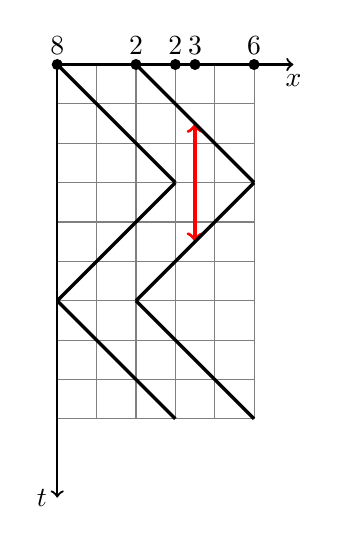
\begin{tikzpicture}
			\draw [help lines,thin,step=5mm] (0,-4.5) grid (2.5,0);
			\draw[thick, ->] (0,0) -- (3,0) node [below] {$x$};
			\draw[thick, ->] (0,0) -- (0,-5.5) node [left] {$t$};

			\fill ( 0   , 0) coordinate (c1) circle (2pt) node [above] {8};
			\fill ( 1   , 0) coordinate (c2) circle (2pt) node [above] {2};
			\fill ( 1.5 , 0) coordinate (c3) circle (2pt) node [above] {2};
			\fill ( 1.75, 0) coordinate (c4) circle (2pt) node [above] {3};
			\fill ( 2.5 , 0) coordinate (c5) circle (2pt) node [above] {6};

			\draw[very thick,red,<->] (1.75,-0.75)--(1.75,-2.25);

			\draw[very thick,-] ( 0  , 0  )--( 1.5,-1.5);
			\draw[very thick,-] ( 1.5,-1.5)--( 0  ,-3  );
			\draw[very thick,-] ( 0  ,-3  )--( 1.5,-4.5);
			\draw[very thick,-] ( 1  , 0  )--( 2.5,-1.5);
			\draw[very thick,-] ( 2.5,-1.5)--( 1  ,-3  );
			\draw[very thick,-] ( 1  ,-3  )--( 2.5,-4.5);
		\end{tikzpicture}
	\end{minipage}

	\begin{minipage}{0.5\hsize}
		\centering
		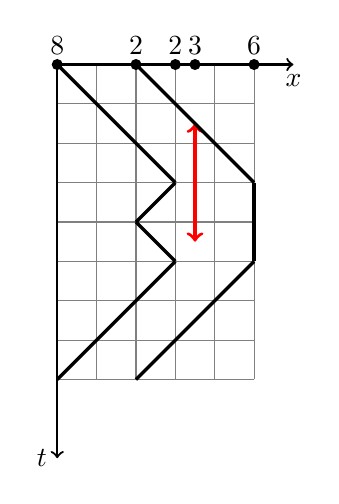
\begin{tikzpicture}
			\draw [help lines,thin,step=5mm] (0,-4) grid (2.5,0);
			\draw[thick, ->] (0,0) -- (3,0) node [below] {$x$};
			\draw[thick, ->] (0,0) -- (0,-5) node [left] {$t$};

			\fill ( 0   , 0) coordinate (c1) circle (2pt) node [above] {8};
			\fill ( 1   , 0) coordinate (c2) circle (2pt) node [above] {2};
			\fill ( 1.5 , 0) coordinate (c3) circle (2pt) node [above] {2};
			\fill ( 1.75, 0) coordinate (c4) circle (2pt) node [above] {3};
			\fill ( 2.5 , 0) coordinate (c5) circle (2pt) node [above] {6};

			\draw[very thick,red,<->] (1.75,-0.75)--(1.75,-2.25);

			\draw[very thick,-] ( 0  , 0  )--( 1.5,-1.5);
			\draw[very thick,-] ( 1.5,-1.5)--( 1  ,-2  );
			\draw[very thick,-] ( 1  ,-2  )--( 1.5,-2.5);
			\draw[very thick,-] ( 1.5,-2.5)--( 0  ,-4  );

			\draw[very thick,-] ( 1  , 0  )--( 2.5,-1.5);
			\draw[very thick,-] ( 2.5,-1.5)--( 2.5,-2.5);
			\draw[very thick,-] ( 2.5,-2.5)--( 1  ,-4  );
		\end{tikzpicture}
	\end{minipage}

	\end{tabular}
	\caption{巡査の協力が必要な例 \label{tikz:multiAgentExample2}}
	% 「可能な限り右に手伝いに行く」戦略が失敗する例
\end{figure}


\red{ここでは「間隔は厳密だが剰余の指定なし」に関する結果はないのだから、二段階に分けて説明する必要がないのでは。つまり、いきなり「間隔は厳密で、剰余の指定あり」の状況、あるいは更に定理2.4の状況に飛んだ方がすっきりするのでは。→}そこで我々は
{\timelimit}の代わりに「{\interval}」というものを考え,
各頂点を警備するにはその点の{\interval}ちょうどごとの時刻には訪問しなければならないという問題も考えた.
この「あえて短い間隔で訪問する」ことで得をしにくいような設定では,
さらに各頂点を訪問しなければならない最初の時刻も指定されるならば,
「できる限り右の方へ動く戦略」で
Lineの全点警備可能性を判定するができることを示した.
実際にはより一般的に,
Line上の訪問しなければならない座標と時刻のペアが有限個指定されている場合について
全点警備可能性判定問題を解くことができる.



\begin{theo}
	\label{theo:LineExactFinite}
	グラフの形状がLineで,
	各頂点$x_i$に対し訪問しなければならない時刻
	$t_{i,1}, t_{i,2}, \ldots, t_{i,{N_i}}$が指定されているとき,
	\red{$(t,x)$の集合?}
	「できる限り右の方へ動く戦略」で巡査を左側から1人ずつ割り当てることで
	全点警備可能性判定問題を解くことができる.
\end{theo}


「できる限り右の方へ動く戦略」は,次のように定義する.

% 定義
まず,図\ref{tikz:defLR}のように$t$-$x$平面の点$a = (t_a,x_a)$に対して領域$L(a), R(a)$を
\begin{align*}
	R(a) &:= \setmid{(t,x)}{ -x + x_a + t_a < t < x - x_a + t_a } \\
	L(a) &:= \setmid{(t,x)}{ (t,x) \not\in R(a) }
\end{align*}
と定義する.
$R(a),L(a)$を$R(t_a,x_a),L(t_a,x_a)$のようにも書くことにする.

\begin{figure}[h]
	\centering
	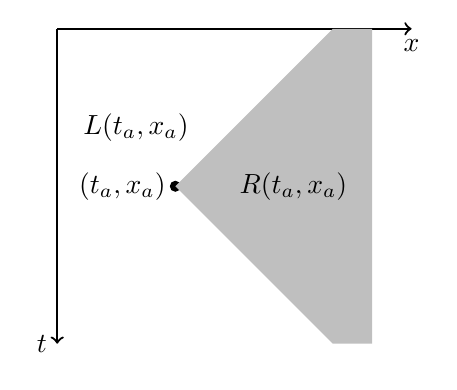
\begin{tikzpicture}
		% \draw [help lines, thin,step=10mm] (0,-5.5) grid (5.5,0);
		\draw[thick, ->] (0,0) -- (4.5, 0) node [below] {$x$};
		\draw[thick, ->] (0,0) -- (0,-4) node [left] {$t$};

		\fill ( 1.5,-2) coordinate (a) circle (2pt) node [left] {$(t_a,x_a)$};

		\fill [fill=lightgray]
			(a)--(3.5,0)--(4,0)--(4,-4)--(3.5,-4)--(a);

		\node (L) at (1,-1.25) {$L(t_a,x_a)$};
		\node (R) at (3,-2) {$R(t_a,x_a)$};
	\end{tikzpicture}
	\caption{$L(t_a,x_a)$ と $R(t_a,x_a)$ の定義 \label{tikz:defLR}}
\end{figure}



$t$-$x$平面上の点の集合$X'$が与えられたとき,
$X'$のどの点$a$に対する右側の三角形の領域$R(a)$にも含まれない領域
$\dbigcap_{a \in X'} L(a)$の(右の)境界線が軌跡であるような動き方を「できる限り右の方へ動く戦略」と定義する.
%
定理\ref{theo:LineExactFinite}は,
与えられた巡査のうち一番左を動く巡査$s_1$が(初期順序を保つ動き方において)どのような動き方をしたとしても
「できる限り右の方へ動く戦略」で$s_1$が訪問する点の一部しか訪問できないという意味で
「できる限り右の方へ動く戦略」は$s_1$の最適な動き方であり,
この動き方で1人ずつ巡査の動きを左側から定めることができるので巡査の必要最小数が分かるという主張である.

\red{ここを編集中}



\begin{proof}[証明\red{←何の?}]
全頂点を警備する任意の順序保存運行$A$で一番左側を動く巡査$s_1$の軌跡を考える.
%
もし$t$-$x$平面上のある点$(t_a,x_a)$から定まる$R(t_a,x_a)$に含まれる点$(t_b,x_b)$を
$s_1$の軌跡が通っているとすると,
$s_1$は$|x_a - x_b| > |t_a - t_b|$より時刻$t_a$に座標$x_a$を訪問できないので
$s_1$が一番左側を動くことから$(t_a,x_a)$が訪問されない点となってしまい矛盾する.
%
よって,$A$で一番左側を動く巡査$s_1$の軌跡は$\dbigcap_{a \in X'} L(a)$に含まれる.
$L(X') := \dbigcap_{a \in X'} L(a)$とする.

一方,この領域$L(X')$の境界線は傾き$1$または$-1$の線分のつながったものであるので,
$s_1$はこの境界線が軌跡となるように動くことができ,
そのようにすることで$L(X')$に含まれるすべての点を訪問でき
$A$での$s_1$の動きを改善できる.
%
$s_2, s_3, \ldots, s_m$の動き方も$X'$ の残りの点に対して
$s_1$のときと同様に決めていくことで$A$での動きを改善できる.

\red{ここを編集中}

\end{proof}









\section{Star}
グラフの形状がStarの場合については,
利得か{\timelimit}のいずれかが一般であれば,
{\patrolling}は巡査が1人であってもNP困難であることがわかっている\cite{coene2011charlemagne}.
そこで,ここでは巡査数が一般であって,
利得と{\timelimit}がすべて等しい場合を考える.
巡査同士が協力をしない設定では,
{\decisionpp}に相当する問題\red{←定義?}でこの場合がNP困難になることが
Coeneら\cite{coene2011charlemagne}により示されているが,
協力を許す設定では多項式時間で解くことができる.

\begin{theo}
	\label{theo:StarEqualProfitTimelimit}
	グラフの形状がStarで利得と{\timelimit}がすべて等しい場合,
	{\patrolling}は多項式時間で解くことができる.
\end{theo}


\begin{proof}[証明]
	\red{編集中}

	巡査数を$m$, 全頂点の{\timelimit}を$Q$, 頂点$v_i$に接続する枝を$e_i$, その長さを$d_i$とする.

	まず,$d_i > Q/2$であるような頂点$v_i$は,警備するならば巡査が1人常駐するとしてよい.
	これは次のように示される.
	%
	(i)ある運行において$v_i$が1人の巡査$s$により単独警備されるとすると,
	$v_i$を訪問してから別の頂点$v_j$を訪問して再び$v_i$に戻ってくるには$2d_i$以上の時間がかかり
	$2d_i > Q$より$v_i$が警備できなくなってしまうため$v_i$以外の頂点を警備することができないので
	$v_i$のみを警備すればよく,これは$v_i$に常駐すれば十分である.
	%
	(ii)もし$v_i$が2人以上の巡査により警備されるとすると,
	ある巡査$s_a$が時刻$t_a$に$v_i$を訪問してから時間$Q$以内の時刻$t_b$に
	別の巡査$s_b$が$v_i$を訪問するという状況が発生するが,
	$s_a$が枝
	$s_b$は端点$v_i$を含む枝$e_i$上のある点に同時に存在するような時刻が
	$s$が
	$s$は$s'$とすれ違うことなく$v_i$以外の頂点を訪問



	2人の巡査がすれ違う動きは互いに動きを交換して引き返す動きに変換しているとすると
	$s$と$s'$が枝$e_i$上で1度以上すれ違わない限り$s'$が$v_i$を訪問するときには$s$も
	$v_i$を訪問しているので,
	$v_i$は$s$のみにより警備できており,$s$も$v_i$以外を警備していない動きとなる.


	また,全頂点は利得と{\timelimit}がすべて等しいので,
	枝の短い頂点から選んでよい.
	実際,ある警邏において警備している頂点$v_i$と警備していない頂点$v_j$であって
	枝の長さが$d_i > d_j$となっているようなものがあったとき,
	$v_j$を訪問していた時刻に代わりに$v_i$を訪問するようにすべての巡査の動きを変えることができる.


	よって,あとは隣接している枝の短い頂点から何個の頂点を選べるかを計算できればよい.
	%
	はじめに,頂点を枝の長さの昇順でソートし,枝の短いものから順に$v_1,v_2, \ldots, v_n$とする.
	これらを枝の長さが$Q/2$以下のグループ$V_1 = \set{v_1, \ldots, v_k}$と
	それ以外のグループ$V_2 = \set{ v_{k + 1}, \ldots, v_n }$に分ける.
	$V_2$の頂点は,$V_1$の全頂点を$m - 1$人以下の巡査により警備できる場合のみ,
	残りの巡査の人数分$V_2$の頂点を選び1人ずつ巡査を常駐させることで警備すればよいので,
	まず$V_1$のすべての頂点を警備できる最小の巡査数$m'$を求める必要がある.

	$m' \leq m$であれば利得(警備できる頂点数)は$k + (m - m')$となる.
	$m' > m$であれば$V_1$のうち

\end{proof}












\section{\unit}

% 完全グラフの場合は巡査が1人でもNP困難であることが示されていたので
定理\ref{theo:StarEqualProfitTimelimit}からStarの特殊な場合とみなせる{\unit}も
巡査1人で利得と{\timelimit}がすべて等しい場合は{\patrolling}がPであることがすぐに分かるが,
{\timelimit}さえすべて等しければ巡査数と利得が一般の場合でも{\patrolling}がPとなる.
%
これは,警備のコストとなる辺の長さと{\timelimit}の両方が全点で等しいことによって
単純に利得の大きい頂点から選べばよいためである.



\subsection{{\timelimit}がすべて等しい場合}




\subsection{{\timelimit}が一般の場合}



{\unit}で{\timelimit}がすべて等しい場合はPであることを示せたが,
{\timelimit}が一般の場合は多項式時間アルゴリズムやNP困難性を示すのが難しかったため,
ここでもLineのときのように,
最初の訪問時刻からその{\interval}ごとの時刻は必ず訪問しなければならないという問題をここでも考えてみる.



\red{
	1. 最初の訪問時刻も指定されるときの{\patrolling}は独立点集合問題からの帰着でNP困難. \\
	2. 全点警備可能性判定なら1人のときはP(おまけ). \\
	3. 最初の訪問時刻が指定されず自由度がある場合は
	   Disjoint Residue Class Problem と同じ問題になるのでNP困難(おまけ).
}





\subsubsection{{\interval}の場合}
{\timelimit}を{\interval}に替えた問題では
巡査が1人の場合でも{\unit}上での{\decisionpp}がNP困難となる.

\begin{theo}
	\label{theo:Comp_exact_NPhard}
	グラフの形状が{\unit}で,
	{\interval}が与えられたときに,
	最初の訪問時刻からその{\interval}ごとの時刻は必ず訪問しなければならないという制約の場合,
	巡査が1人でも{\decisionpp}がNP困難である.
\end{theo}

\begin{proof}[証明]
	Disjoint Residue Class Problem~\cite{kawamura2015simple}からの帰着による.

	ある整数のペアの集合 $\set{ (m_1, r_1), \ldots, (m_n, r_n) }$ が
	Disjoint Residue Class であるとは,
	任意の整数 $x$ に対して $x \equiv r_i \mod m_i$ となるような $i$ が
	高々1つ存在することと定義される.
	Disjoint Residue Class Problem とは
	整数の組 $(m_1, \ldots, m_n)$ が与えられたときに,
	$\set{ (m_1, r_1), \ldots, (m_n, r_n) }$ が
	Disjoint Residue Class となるような組 $(r_1, \ldots, r_n)$ が
	存在するかを判定する問題であり,
	これはNP困難であることが知られている~\cite{kawamura2015simple}.

	Disjoint Residue Class Problem は,
	巡査1人,グラフの形状が{\unit}で
	{\interval}ごとの時刻は必ず訪問しなければならないという制約での{\decisionpp}に多項式時間帰着できる.
	Disjoint Residue Class Problem の入力が $(m_1, \ldots, m_n)$ のとき,
	{\unit}で頂点を$V = \set{ v_1, \ldots, v_n }$, {\interval}を$q_i = m_i$, 辺の長さを$d = 1$ とする.
	$d = 1$ より整数の時刻にいずれかの点を訪問できるようにする.
	各頂点 $v_i$ の最初の訪問時刻を $r_i$ とすると,
	この点を警備するために訪問しなければならない時刻の列は
	$q_i k + r_i (k \in \N)$ で与えられるが,
	全点を警備するためには任意の2点 $v_i, v_j \in V$ , 任意の整数 $k,l$ について
	$q_i k + r_i \neq q_j l + r_j$
	である必要がある.

	% Disjoint Residue Class Problem が Yes ならば \decisionpp も Yes
	Disjoint Residue Class Problem の解 $(r_1, \ldots, r_n)$ が存在するならば,
	これにより任意の時刻 $t \in \Z$ に対して $t \equiv r_i \mod q_i$, 
	すなわち $t = r_i + q_i k$ となる $k \in \Z$ が存在するような $i$ は高々1つであり,
	任意の $k,l \in \Z$ に対して $q_i k + r_i \neq q_j l + r_j$ が成り立つので,
	巡査は全点を警備できる.

	% \decisionpp が Yes ならば Disjoint Residue Class Problem も Yes
	逆に{\decisionpp}の解が存在するとき,
	全点を警備できるのでその警邏において各頂点$v_i$を最初に訪問する時刻を $r_i$ とすると,
	任意の $v_i,v_j \in V$, $k,l \in \Z$ に対し
	\begin{equation}
		\label{eq:patrollDisjoint}
		q_i k + r_i \neq q_j l + r_j
	\end{equation}
	が成り立つ.すると,任意の時刻 $t \in \Z$ に対して
	$t \equiv r_i \mod q_i$ となるような $i$ が2つ存在するとすると,
	それを $i$, $j$ として
	$t \equiv r_i \mod q_i$, $t \equiv r_j \mod q_j$
	すなわち,ある整数 $k,l$ が存在して
	$t = q_i k + r_i$, $t = q_j l + r_j$
	となり,この $k,l$ によって
	$q_i k + r_i = q_j l + r_j$ となり,式\ref{eq:patrollDisjoint} に矛盾する.
	よって,任意の整数 $t$ に対して $t \equiv r_i \mod q_i$ を満たす
	$i$ は高々1つであるような $r_i$ が与えられたので,
	{\decisionpp}の解が存在するとき,
	Disjoint Residue Class Problemにも解が存在する.

	以上よりDisjoint Residue Class Problemを帰着できた.
\end{proof}







\subsubsection{最初の訪問時刻指定,{\interval}}
今,最初の訪問時刻には自由度があり{\interval}だけが指定される問題を考えたが,
さらに最初の訪問時刻も与えられる問題も考えることができる.

\begin{theo}
	\label{theo:UnitSingleExactStarttime}
	グラフの形状が{\unit}で巡査が1人の場合,
	最初の訪問時刻と{\interval}が与えられて
	最初の訪問時刻からその{\interval}ごとの時刻は必ず訪問しなければならないという問題の場合,
	{\decisionpp}はPである.
\end{theo}

\begin{proof}[証明]
	まず,{\unit}の辺の長さを$d$とする.
	各$i$について正整数$q _i$と整数$r _i$とが与えられ,
		集合$S _i = \{\, q_i k + r_i : k \in \Z \,\}$に属する時刻に
		頂点$v _i$を訪問することが要求される.
	\red{(定義済?→)}{\decisionpp}がYesである(=全頂点を警備できる)ことは,
	連続した訪問しなければならない時刻の差がすべて移動時間$d$以上であること,すなわち
	任意の相異なる$i$,$j$について
		$S _i$に属するどの時刻と
		$S _j$に属するどの時刻も差が$d$以上であることを意味する.
	これは任意の2頂点$v_i, v_j \in V$と
	任意の整数$k,l$に対して$\abs{ (q_i k + r_i ) - (q_j l + r_j) } \geq d$という条件となり\red{(←「$(i, k) = (j, l)$の場合を除いて」が必要?)},これは
	任意の整数$n$に対して$\abs{ (r_i - r_j) + gcd(q_i, q_j) n } \geq d$と同値であり,
	左辺の最小値を考えると
	$\abs{ r_i - r_j }$を$gcd(q_i, q_j)$で割った余り$a$と
	$gcd(q_i, q_j) - a$ のうち小さい方が$d$以上かを計算すればよい.
	この計算は定数時間であり
	${}_n C_2$ 通りこれを調べればよい.
\end{proof}




{\decisionpp}で巡査を複数とすると,$T$ に差が $d$ 未満の整数が含まれていても
複数の巡査によりそれぞれ訪問できる場合が生じるため難しい.



{\decisionpp}では巡査が1人ならば多項式時間アルゴリズムが存在したが,
一方{\patrolling}は巡査が1人でも(複数人でも)NP困難となる.

\begin{theo}
	\label{theo:UnitExactStarttimeNPhard}
	グラフの形状が{\unit}で,
	最初の訪問時刻と{\interval}が与えられたときに,
	最初の訪問時刻からその{\interval}ごとの時刻は必ず訪問しなければならないという問題の場合,
	巡査が1人で利得がすべて等しい場合でも{\patrolling}はNP困難である.
\end{theo}


\begin{proof}[証明]
	最大独立点集合問題からの帰着による.

	最大独立点集合問題は,
	無向グラフ$G = (V, E)$が与えられたときに
	独立点集合で最大のものを求める問題でNP完全であることが知られている.
	この問題において,間に辺の存在する2頂点の両方を選ぶことはできないという制約を,
	{\patrolling}において2頂点のどちらか一方しか警備できないという制約に帰着する.

	まず{\unit}の辺の長さを$d = 1$とする.
	これにより巡査がちょうど速さ$1$で動くとすると各頂点の訪問にかかる時間は$1$となり,
	{\unit}なのですべての整数の時刻にどれか1点を訪問できる.
	その上で,{\interval} $q_i$, 最初の訪問時刻 $r_i$ は整数,利得はすべて1とする.
	{\unit}の頂点集合は$V$とする.
	頂点$v_i$を警備するために訪問しなければならない時刻の列は
	$q_i k + r_i \; (k \in \N)$ で表される.
	すると,$v_i$ と $v_j$ の両方を警備できる必要十分条件は
	\[ q_i k + r_i = q_j l + r_j \]
	すなわち
	\[ r_i - r_j = q_j l - q_i k \]
	となる自然数 $k, l$ が存在しないこととなるが,
	これは $r_i - r_j = gcd(q_i,q_j) n$ となる整数 $n$ が存在しないことと同値である.
	よって,
	$v_i$ と $v_j$ の両方を警備できる必要十分条件は
	$r_i \not\equiv r_j \mod gcd(q_i, q_j)$
	となる.

	ここで,${}_n C_2$ 個の相異なる素数 $p_{ij} (1 \leq i < j \leq n)$ を用意し,
	各頂点の{\interval}を
	$q_i = p_{1i} p_{2i} \cdots p_{(i - 1)i} p_{i(i + 1)} \cdots p_{in}$
	とすると,$gcd(q_i,q_j) = p_{ij}$ ($i < j$ のとき)となり,
	先ほどの条件は
	$r_i \not\equiv r_j \mod p_{ij}$
	となる.

	$G$ において
	$(v_i, v_j) \in E$	 ならば $r_i \equiv r_j \equiv 0 \mod p_{ij}$,
	$(v_i, v_j) \not\in E$ ならば $r_i \equiv 0, r_j \equiv 1 \mod p_{ij}$
	と定めると,
	各 $r_k$ に対して相異なる $n - 1$ 個の素数で割ったときの余りが与えられるので,
	中国剰余定理からそのような $r_k$ がその $n - 1$ 個の素数の積 $q_k$ を法として一意に存在することが言え,
	これにより,$(v_i, v_j) \in E$ ならば $r_i \equiv r_j \mod p_{ij}$
	$(v_i, v_j) \not\in E$ ならば $r_i \not\equiv r_j \mod p_{ij}$
	を満たすように各 $r_k$ を定めることができる

	最後に,${}_n C_2$ 個の相異なる素数を用意する計算量も確かめる必要がある.
	$k$ 番目に小さい素数を $P_k$ と書くと,$k \geq 6$ のときは
	$P_k < k( \ln k + \ln\ln k )$ であることが知られているため~\cite{dusart1999k},
	$k( \ln k + \ln\ln k )$ までの自然数を順に素数かどうか判定していくことで
	$k$ 個以上の素数を得ることができる.
	ある数が素数であるかどうかを判定する多項式時間アルゴリズムは存在するので~\cite{agrawal2004primes},
	${}_n C_2$ 個の素数の列挙は$n$の多項式時間でできる.

	以上の手順で $q_k$ と $r_k$ を設定することにより,
	$G$ において最大の独立点集合を求める問題を,
	最初の訪問時刻が指定され周期ちょうど毎に訪問しなければならない問題で
	巡査が1人で利得がすべて等しい場合の{\patrolling}に帰着できた.
\end{proof}
